\chapter{3er semana - Variables y Compoteras}

\nota{Introducción}{En la segunda semana aprendimos sobre cómo hacer para mostrar por pantalla números y cadenas y vimos qué pasaba si las sumás, si las multiplicás y demás}
\nota{Objetivo}{El paso que queremos dar es empezar a almacenar información, para esto vamos a usar un concepto que es realmente muy importante que se llama \emph{variable}}
\nota{Cómo lo vamos a hacer}{Vamos a mostrar cómo utilizar las variables de la forma más sencilla posible en diferentes programas, siempre usando los conceptos que aprendimos antes}

\section{Introducción}
Hasta ahora, cada vez que hacíamos una cuenta, una operación de sumas o simplemente cuando mostrábamos algo por pantalla no teníamos manera de saber en dónde almacenar esta información, la usábamos una vez y luego la perdíamos.\\

Por ejemplo, si queremos que el programa imprima por pantalla las palabras “hola, como andas” muchas veces teníamos que hacer:

\begin{lstlisting}
puts ' ...hola, como andas..'
puts ' ...hola, como andas...'
puts ' ...hola, como andas...'
puts ' ...hola, como andas...'
\end{lstlisting}

Estaría bueno poder guardar el valor en algún lado (en la memoria de la compu) y después usarlo cuando tenemos ganas, ¿no?.
 
\section{Variables}
Para poder guardar una cadena en un lado le tenemos que poner un nombre. Los programadores decimos a esto asignación y los nombres que usamos se llaman variables. Como nombre o variable podemos usar cualquier combinación de letras que queramos. La única condición es que el primer carácter tiene que ser una letra en minúscula. Vamos a probar el programa anterior pero ahora usando una variable para guardar el valor de la cadena que queremos imprimir por pantalla, le vamos a poner como nombre: mi\_cadena.

\begin{lstlisting}
mi_cadena = ' ...hola, como andas..'
puts mi_cadena
puts mi_cadena
\end{lstlisting}

Ahora ejecutémoslo y veamos que resulta...
Así, cada vez que queramos hacer algo con mi\_cadena, Ruby va a usar el valor que está guardado en mi\_cadena. Una manera de verlo es que mi\_cadena apunta un valor concreto.\\

En resumen, la variable se llama “mi\_cadena” y el valor es “…hola, como andas…”

\begin{center}
\begin{tabular}{|c|c|}
\hline
\rowcolor[gray]{0.9}Nombre & Valor \\
\hline
mi\_cadena & '…hola, como andas…' \\
\hline
\end{tabular}
\end{center}

Vamos con un ejemplo más copado:

\begin{lstlisting}
mi_nombre = 'Charly'
mi_apellido = 'Lizarralde'
puts 'Yo me llamo ' + mi_nombre + '  y mi apellido es ' + mi_apellido
\end{lstlisting}

Si ejecutamos esto el programa mostraría por pantalla lo siguiente:

\begin{lstlisting}
Yo me llamo Charly y mi apellido es Lizarralde
\end{lstlisting}

Otra cosa que podemos hacer es asignar a una variable un valor y después ¡cambiárselo! Por ej: 

\begin{lstlisting}
mi_nombre = 'Charly'
puts 'Yo me llamo ' + mi_nombre
mi_nombre = 'Mariano'
puts 'El se llama ' + mi_nombre
\end{lstlisting}

Además, una variable puede apuntar a cualquier cosa, no solo cadenas... ¡También números! 

\begin{lstlisting}
cualquier_cosa = 'Charly'
puts ' Esto es una cadena ' + cualquier_cosa
cualquier_cosa = 2*4 + 12
puts 'Esto es un numero ' + cualquier_cosa
\end{lstlisting}

Probemos el programa anterior... ¡aunque creo que a esta altura ya nos podemos imaginar que hace!\\

Otra cosa más. Es la última: las variables pueden apuntar a cualquier cosa, pero ¿qué pasa si queremos que apunten a... OTRA VARIABLE?   A ver, probemos...

\begin{lstlisting}
var1 = 8
var2 = var1
puts var1
puts var2
puts ' '
var1 = ' ocho'
puts var1
puts var2
\end{lstlisting}

Esto imprimiría... 

\begin{lstlisting}
8
8

ocho
8
\end{lstlisting}

En la segunda línea, tratamos de apuntar var2 a var1 pero en realidad apunto al 8 que era el valor al cual apuntaba var1. Después cambiamos var1 para que apunte al valor 'ocho'. Cuando imprimimos ambos valores con \emph{puts}, ¡vemos que var2 no cambio!. Lo que pasa, es que var2 nunca apuntó a var1 sino al valor que apuntaba var1 en el momento de la asignación que era 8. Por eso var2 se quedo apuntando al 8. Esto es medio difícil de entender así como así, por eso vemos en el siguiente gráfico como es la cosa.

\begin{center}
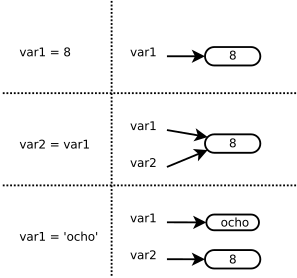
\includegraphics[width=0.5\textwidth]{cap03_fig01}
\end{center}

\section{Ejercicios}
\begin{ejercicio}{Variables}{
\begin{enumerate}
  \item Si queremos hacer una calculadora que sume y reste los mismos números a la vez ¿Cuántas variables necesitamos?
  \item Escribí el programa de arriba
  \item Hacé un programa que imprima por pantalla los siguientes números: 1 2 4 8 16 32, pero usando variables
  \item Hacé un programa que permita al usuario ingresar una palabra y la multiplique por 15
  \item Hacé un programa que me pregunte cuantas veces quiero ver la frase “¡aguante el rojo!” y lo repita por pantalla tantas veces como haya elegido
\end{enumerate} 
}
\end{ejercicio}
